\section{Feasibility of Learning}
\noindent
{\color{LightRubineRed} \rule{\linewidth}{1mm} }

\subsection{No Free Lunch}
Learning from $D$ (to infer something outside$D$) is doomed if any 'unknown' $f$ can happen. :( \par

\subsection{Inferring something} % (fold)
\begin{center}
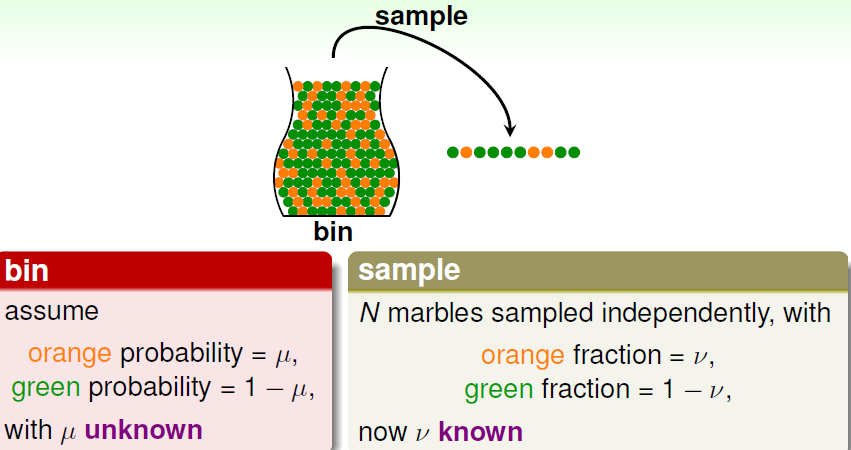
\includegraphics[width=10cm, height=6.5cm]{lecture4_1}\\
\end{center}
\textbf{Hoeffding's Inequality} \par
坏事情发生的几率有多大 \par
\begin{align*}
\mathbb{P}[|\nu-\mu| > \epsilon] \leq 2\exp(-2\epsilon^2N)
\end{align*}
跟$\mu$无关,跟$N$有关,如果样本够多,大概可以去近似。 \par
\subsection{Connection to Learning} % (fold)
\begin{align*}
E_{out}(h) &= \underset{x \sim P}{E} \llbracket h(x) \neq f(x) \rrbracket\\
E_{in}(h) &= \frac{1}{N}\sum_{n=1}^N \llbracket h(x) \neq f(x) \rrbracket \\
\end{align*}
$E_{in}$in-of-sampling(Known) \\
$E_{out}$out-of-sampling(UnKnown) \\
就像刚才一样我们不需要知道$E_{out}$,只需要$N$足够大即可。\par
\begin{align*}
\mathbb{P}[|E_{in}-E_{out}| > \epsilon] \leq 2\exp(-2\epsilon^2N)
\end{align*}
这样从理论保证,对于固定的$h$,如果数据足够多的话。
\begin{align*}
	E_{in} \approx E_{out}
\end{align*}
\subsection{Multiple h} % (fold)
Bound of Bad data \par
\begin{align*}
%http://ccxxxx.blog.51cto.com/7769075/1339606
\mathbb{P}_D[\text{bad} \ \mathcal{D}] \\
&= \mathbb{P}_D[\text{bad} \ \mathcal{D} \; for \; all \; h] \\
&\leq 2M\exp{-2\epsilon^2N}
\end{align*}
如果算法$A$找到一个$g$保证$E_{in} \approx 0$,那么理论保证$E_{out} \approx 0$ \\
$M$应该代表了复杂度,$N$代表了数据多少,理解这两个数值对ML的优化很有帮助。 
\begin{center}
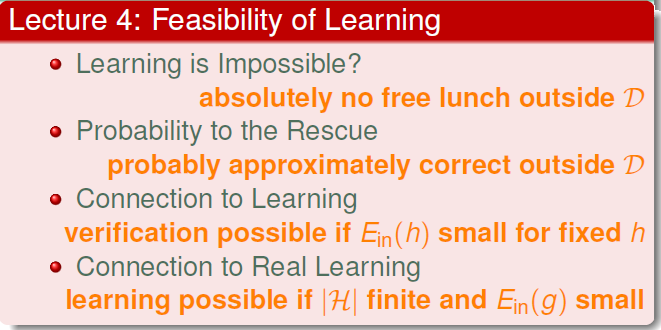
\includegraphics[width=10cm, height=6cm]{lecture4_sum}
\end{center}
\noindent
{\color{RubineRed} \rule{\linewidth}{1mm} }
